%%%%%%%%%%%%%%%%%%%%%%%%%%%%%%%%%%%%%%%%%%%%%%%%%%%%%%%
% A template for Wiley article submissions.
% Developed by Overleaf.
%
% Please note that whilst this template provides a
% preview of the typeset manuscript for submission, it
% will not necessarily be the final publication layout.
%
% Usage notes:
% The "blind" option will make anonymous all author, affiliation, correspondence and funding information.
% Use "num-refs" option for numerical citation and references style.
% Use "alpha-refs" option for author-year citation and references style.
\documentclass[alpha-refs]{wiley-article}
%\documentclass[blind,alpha-refs]{wiley-article}
\usepackage{xcolor}
\usepackage{siunitx}
\usepackage{apalike}
\usepackage{gensymb}
\usepackage{makecell}
\usepackage{csquotes}
\usepackage{graphicx}
\usepackage{listings}
\usepackage[T2A]{fontenc}
\usepackage[utf8]{inputenc}
\usepackage[english]{babel}
\usepackage[version=3]{mhchem}
%\usepackage{amsmath,amsfonts,amssymb,amsthm,mathtools} % AMS

\papertype{Original Article}

\title{Cytoskeletal and motility changes in human umbilical cord mesenchymal stem cells associated with nuclear-cytoplasmic RhoА redistribution during replicative senescence}


% List abbreviations here, if any. Please note that it is preferred that abbreviations be defined at the first instance they appear in the text, rather than creating an abbreviations list.
\abbrevs{MSCs, mesenchymal stem cells; RCF, relative centrifugal force; }

% Include full author names and degrees, when required by the journal.
% Use the \authfn to add symbols for additional footnotes and present addresses, if any. Usually start with 1 for notes about author contributions; then continuing with 2 etc if any author has a different present address.
\author[1\authfn{1}]{Danila Bobkov}
\author[2\authfn{2}]{Anastasia Polyanskaya}
\author[1\authfn{1}]{Anastasia Musorina}
\author[1\authfn{1}]{Ekaterina Lomert}
\author[1\authfn{1}]{Sergey Shabelnikov}
\author[1\authfn{1}]{Galina Poljanskaya}

% \contrib[\authfn{1}]{Equally contributing authors.}

% Include full affiliation details for all authors
\affil[1]{Institute of Cytology of the Russian Academy of Science, 194064 Tikhoretsky ave. 4, St-Petersburg, Russia }
\affil[2]{Peter the Great St. Petersburg Polytechnic University, Polytechnicheskaya, 29,  St.Petersburg, 195251, Russia}

\corraddress{Tikhoretsky ave. 4, St-Petersburg, 194064, Russia}
\corremail{bobkov@incras.ru}

\presentadd[\authfn{2}]{Peter the Great St. Petersburg Polytechnic University, Polytechnicheskaya, 29,  St.Petersburg, 195251, Russia}

\fundinginfo{This research received no external funding.}

% Include the name of the author that should appear in the running header
\runningauthor{Bobkov et al. Motility changes in aging MSCs}

\begin{document}

\maketitle

\begin{abstract}

One of the essential signs of replicative aging is a decrease in cell motility.
Here we provide evidence for changes in the organization of the contractile apparatus of human mesenchymal stem cells in the process of replicative senescence.
The colocalization dynamics of  of myosin-9, alpha-actinin-4, RhoA with F-actin and nuclei were studied at various passages during long cultivation of MSCs.
We demonstrated, for the first time, replicative senescence in connection with RhoA nuclear-cytoplasmic redistribution.
Using the automated system of intravital confocal microscopy, the characteristics of cell motility at various passages were studied.
It was found that during replicative senescence in MSCs, a decline in cell speed and path tortuosity occurs.


% Please include a maximum of seven keywords
\keywords{mesenchymal stem cells, \emph{cellular senescense}, actin cytoskeleton, myosin-9, $\alpha$-actinin-4, RhoA, cell motility}
\end{abstract}

\section{Introduction}

At present, the urgent task of cell biology is the isolation and comparative characterization of human MSCs isolated from various sources.
The importance of such studies stems from the features of the interaction of MSCs isolated from different tissues, with their characteristic microenvironment.
The origin or source of the MSC can determine their functional characteristics.
Comparative analysis of the characteristics that are decisive in maintaining the status of MSCs, as well as a number of other characteristics responsible for the most important cellular processes, contributes to the deepening of basic knowledge of human MSCs, which is important both for understanding the mechanisms of biological processes in the cell and for expanding opportunities for using MSCs in regenerative medicine.
Due to the importance of MSCs for the functioning of the body, the mechanisms of MSC interaction with damaged tissues and organs are widely studied.

It has been shown that one of the most important mechanisms of action of various MSCs on damaged tissues is their ability to migrate to these sites and exert a trophic action due to the secretion of bioactive factors that alter the microenvironment of damaged cells and, thereby, improving tissue repair.
At present, the mechanisms of tissue repair using MSCs related to the production of cytokines and paracrine factors are widely discussed in the literature (\cite{phinney2007concise}; \cite{m2011mesenchymal}; \cite{guiducci2011bone}; \cite{gruenloh2011characterization}; \cite{huang2013effects}; \cite{luo2013mesenchymal}; \cite{ando2014stem}; \cite{hendijani2015human}; \cite{hendijani2015effect}; \cite{danieli2016testing}; \cite{julianto2016topical}; \cite{teixeira2017impact}; \cite{vulcano2016wharton}; \cite{zachar2016activation}).


Non-immortalized cell lines undergo a process of replicative senescence.
Replicative senescence is a complex process that can begin at the early passages and gradually increase in the process of long-term cultivation.
It is characterized by a significant decrease or cessation of proliferation, shortening of telomeres, morphological changes, increased $\beta$-galactosidase activity, increased expression of the tumor suppressor genes, decreased DNA repair and antioxidant activity of senescence cells, due to reduced expression of the corresponding genes, decreased differentiation potential, a number of epigenetic changes (\cite{wagner2008replicative}; \cite{kuilman2010essence}; \cite{redaelli2012cytogenomic}; \cite{estrada2013human}; \cite{savickiene2016senescence}; \cite{danisovic2017effect}; \cite{koltsova2018dynamics}; \cite{alessio2018mesenchymal}; \cite{krylova2018isolation}; \cite{niedernhofer2018nuclear}; \cite{truong2018characterization}; \cite{yu2018replicative}).


It is important to emphasize that senescence of MSCs may be associated not only with replicative senescence, which can be traced during prolonged passsenescence of MSCs in vitro, but also with factors external to MSCs.
Senescence mechanisms affect both MSCs and microenvironment.
In this regard, it is the interaction of MSCs and the microenvironment that ensures the age characteristics of MSCs.
One of the essential signs of replicative senescence is a decrease in cell motility or cell migration.
Violation of migration processes contributes to the deterioration of tissue repair (\cite{geissler2012functional}; \cite{bertolo2015vitro}; \cite{turinetto2016senescence}; \cite{zhang2018overexpression}).
Therefore, to use MSCs in regenerative medicine, it is necessary to know the nature of the process of replicative senescence in a particular line.


In order to find out how much cellular senescence can interfere with use of cells in biomedical work, it is important to  it is important to find out to what extent cell mobility is impaired during long-term cultivation.
Cell migration occurs through close contact with the extracellular matrix, on which cells are spread, and depends on the organization of the actin cytoskeleton.
In this regard, it is essential to study the role of senescence in the organization of the cytoskeleton.
Currently, studies on the effect of replicative senescence on cytoskeleton reorganization are at the stage of accumulation of experimental results.
There are a number of works describing molecular mechanisms and functional changes during the reorganization of the cytoskeleton during replicative senescence in different human and animal cell types (\cite{larsen2003phosphatases}; \cite{le2008regulation}; \cite{wang2009protein}; \cite{geissler2012functional}; \cite{ozcan2016unbiased}; \cite{turinetto2016senescence}; \cite{moujaber2019cellular}).

It is of considerable interest to analyze the effect of replicative senescence on cell motility and the reorganization of the actin cytoskeleton in the human MSC line, which has not been used in detail in such studies.
Actin cytoskeleton provide the driving forces for creating morphological diversity and the dynamics of mammalian cells (\cite{vasiliev1991polarization}).
Motor proteins, such as nonmuscle myosin isoforms, involved in maintaining cell shape, cell migration, interaction with the substrate and with other cells, cytogenesis, processes of intracellular transport, as well as signalling and the regulation of gene expression (\cite{omelchenko2002mechanisms}).

Thus, the objective of this study is analysis of replicative senescence in the process of long-term cultivation of the MSCWJ-1 in terms of the actin cytoskeleton structure and the behavior of moving cells.
In this work, we used MSCWJ-1 cells that were not previously investigated.
The hypothesis of this study was that motility changes associated with human MSC senescence are actin-cytoskeleton and RhoA-dependent.

Little is known about how the structural aspects of these cells are modified as a result of replicative senescence.
Using fluorescence and confocal microscopy-based quantitative image cytometry techniques, we investigated changes in distribution of F-actin and actin-binding proteins myosin-9 and $\alpha$-actinin-4 as well as small GTPase RhoA in conjunction with the registration of parameters characterizing cell motility.
In order to characterize the change in the composition of cytoplasmic protein complexes containing myosin-9 and beta-actin, we used liquid chromatography.


\section{RESULTS}

\subsection{$\beta$-Galactosidase activity}

The degree of replicative senescence during long-term cultivation of MSCWJ-1 was assessed by the activity of $\beta$-galactosidase in cell populations.
The results are presented in the table 1.
The proportion of stained cells naturally increases with senescence, which confirms the status of this cell line as senescence non-transformed cells.

\subsection{Immunofluorescent and colocalization analysis}

Morphological analysis of the cell line during long-term cultivation showed homogeneity of cell populations with medium-sized elongated fibroblast-like cells at the 9th and 28th passages.
In the process of cultivation, there was a change in the morphology of the cells, expressed in an increase in the size and degree of cell spreading.
In order to assess the changes in the structure of the contractile apparatus that can occur during replicative senescence, we used the immunofluorescence method.
We used rhodamine-phalloidin for staining F-actin and anti-myosin-9 heavy chain polyclonal antibodies, combination of this staines allowed contrictile apparatus visualization.
Characteristic images shown in Fig. 1.
In all spread cells, staining for myosin-9 reveals a characteristic striated pattern.
Myosin-9 is distributed along stress-fibrils (Fig. 1 B).
In addition to the striated pattern (Fig. 1 C), myosin-9 is detected in lamellae as separate spots (Fig. 1 D).


In order to follow the dynamics of the reorganization of the contractile apparatus during replicative senescence, we analyzed the localization of myosin-9 and F-actin in different passages.
The results are presented in the figure 2.
In the analysis of immunofluorescence images, we calculated five variants of the colocalization coefficients, namely: Kendall's Tau-b rank correlation value (Tau-b), Spearman's rank correlation value (Rs), Manders' M in two varians was get above threshold (tM1 and tM2), and Pearson's R value above threshold (Rval).
We conducted PCA and a show correlation matrix plot in order to identify the coefficient most suitable for our purposes.
It turns out, that bTau and Rs coefficients shows very high correlation.
tM1 and Rval coefficient shows moderate correlation (see supplement for details).
Kruskal-Wallis rank sum test results presened in table (supp 3) suggest that bTau reflects changes in colocalization so well.
The output from factor analysis in R shown in table 2.
The uniqueness is the variance that is unexplained by the factors and is unique to that specific variable.
The factors have different weights for different variables and they are called the loadings.
The PCA and factor analysis allowed us to conclude that bTau is the most suitable coefficient and in the future we use it for the analysis of cytoskeletal rearrangements.


As can be seen in fig 3, A, the colocalization of myosin-9 and F-actin decreases from high to moderate level during cultivation and reaches a minimum at passage 15.
Then, the colocolization rises to a very high level at passage 28, after which it again decreases during passage of cultivation to passage 36, which was our last time point.
The use of post hoc analysis revealed the most significant differences between groups associated with a decrease in colocalization at 15 and 18 passages (fig 2, E).
For further research, we decided that 9, 15, 28, and 36 passages would be key points.


The results of staining cells with alpha-actinin-4 in these passages are presented in Fig. 6.
$\alpha$-Actinin-4 as well as myosin-9 was detected in cells in the form of striated patterns, less pronounced than in myosin-9, but nevertheless quite distinguishable.
We studied the colocalization of actinin with actin, as well as with nuclei.
The results are presented in fig. 6.
At passage 15, spotting is observed in $\alpha$-actinin-4 stained.


As seen from figure 2, A, colocalization of $\alpha$-actinin-4 with nuclei decreases from moderate level to weak when moving from 28 to 36 passages.
The same decrease is observed in the transition from 9 to 15 passage in case of $\alpha$-actinin-4 and F-actin colocalization.


The colocalization of small GTPase RhoA with nuclei significantly increases from moderate to noticeable level while passage gone from 9 to 15, then decreases to the initial level at passage 28, and even more decreases to the weak level at passage 36.
It should be noted that in almost half of the cells, the coefficient takes negative values, which indicates the complete absence of colocalization.


For a more detailed study of the detected phenomenon of nuclear-cytoplasmic shuttle, we used the analysis of 3D models performed in the nuclear region.
Figure 7 shows aRhoA in the nucleus images based on Z-stacks.
In the XZ sections, it is noticeable that at the 9th passage, RhoA is distributed partly in the nucleus and partly in the cytolasm, at the 15th passage for the most part inside the nucleus and in the perinuclear region, and at the 36th passage only along stress fibrils and in the cytoplasm.

\subsection{Trajectory analysis}


In fig.8, A characteristic frames from time laps of cell movement recording over 24 hours are presented.
The results of a statistical analysis of the obtained trajectories are presented in Fig.5, В.
The R script used to perform this analysis is available in the supplement.
Speed and path length significantly decreased with increase in passage number.
At the same time, the total distance traveled significantly decreases only when switching from 9 to 15 passages and 15 passage does not differ from 36.
The straightness of the trajectory increases significantly with the passage from passage 15 to 36.
The tortuosity of the trajectory increases with the transition from passage 9 to 15 and then decreases by passage 36 to a level significantly lower than it was at passage 9.


The numerical values obtained from the analysis of 24-hour cell trajectories are presented in the table \ref{tab3}.

\subsection{Gel chromatography}


Chromatographic analysis showed that myosin-9 was detected at passage 9 in most of its regions in the region of high molecular fractions 3 and 4, and to a lesser extent in fractions 7 and 9 (Fig 6).
At passage 15, the amount of myosin in fractions 3–--4 decreases, but the tail of the elution distribution is enriched: low molecular weight fractions are uniformly colored at a good signal level, starting from 10 to 14.
At passage 36, myosin is detected mainly in 3---4 fractions.


$\beta$-Actin is detected mainly in the 10---11 fractions at passage 9.
But at 15 and 36 passages it also begins to be revealed in fractions 6---7.

\section{DISCUSSION}

The proportion of cells with pronounced activity of $\beta$-galactosidase ($\beta$-gal) in the process of cultivating the MSCWJ-1 line confirm the aging status of cells.
The number of cells stained for galactosidase naturally increases during the long-term cultivation of stem cells.


The actin cytoskeleton and its associated motor protein myosin-9 demonstrate characteristic striated pattern in in all studied passages, but at passages 15-17 among the variants of the spatial organization of the cytoskeleton, a spotty pattern becomes noticeable.

Cytoskeleton isoactins form less stable polymers than skeletal muscle actin \cite{khaitlina2001functional}.

A number of actin-binding proteins prevent the depolymerization of F-actin microfilaments and regulate their stability, such as tropomyosin, alpha-actinin, for example.

In this regard, we decided to see how the interaction of alpha-actinin with actin changes.


Both external and intrinsic factors control directionality of cell movement \cite{tiurin2013molecular}.

We believe that the detected changes in the localization of F-actin and actin-binding proteins reflect the phenomenon of partial disassembly of the cytoskeleton, which is characteristic for switching types of cell movement.

Since myosin-9 is a key protein for cell migration, we investigated the distribution various passages.
It was shown that tropomyosins act as negative regulators of myosin stack formation \cite{hu2019reciprocal}.
This figure of 50 doublings, called the Hayflick limit, is fairly arbitrary, since it is not possible to accurately determine how many times a single human cell can share.

Thus, the results of Hayflick's experiments do not mean that the human cell is able to share exactly 50 times (most likely more), but only mean that with the counting method that Hayflik used and which is used now as the simplest and most convenient, a population of human fibroblasts in culture doubles usually ~ 50 $\pm$ 10 times.

Cell cycle arrest during replicative senescence.



Another structure characteristic mainly of non-muscle cells is stress fibrils — bundles of F-actin filaments stabilized by such proteins.
Features of the organization of the actin cytoskeleton in mesenchymal stem cells.

At present, analogs of bone marrow MSC are found in all other tissues.

Thanks to the approaches that allow identifying MSCs in situ, isolating them from tissues and finally evaluating biological properties, it became possible to revise the role of MSCs in various organs and tissues.

In our opinion, MSCs perform the function of conjugating the circulatory, immune, hormonal, and nervous systems with tissue-specific stem cells.


Elliott et al. find that Rho/ROCK-stimulated myosin II contractility minimizes cell-scale branching by recognizing and minimizing local cell-surface curvature \cite{elliott2015myosin}.

Differences in the organization of the cytoskeleton in normal and cancer cells (\cite{shutova2010normal}).

The cell movement is based on the rearrangement of the actin cytoskeleton. The initial step of the rearrangements is the formation of the so-called leading (active) edge, at which protrusions take place and primary contacts of the cell with the extracellular matrix are formed.

% \cite{gorelik2014quantitative}

Protrusion of the leading edge is provided by the force of polymerization of actin in the zone of the lamellipodia. In the lamella zone, a further rearrangement of actin takes place - the formation of actin-myosin beams.

The formation of contacts with the substrate is initiated in the lamellipodia, and maturation occurs in the lamella zone with the participation of stress-fibrils (Alexandrova et al., 2008).


The tension generated by myosin affects the initial focal complexes, inducing their growth and transformation into focal contacts (Ingber, 1991; Riveline et al., 2001; Rottner et al., 2001; Krendel, Mooseker, 2005).

A striking example of the dynamic organization of the cytocell is its restructuring, occurring in the cell spreading process.
The process of spreading begins with the formation of pseudopodia around the entire perimeter of the cell.
The network of microfilaments on the active edge is constantly formed during the entire spreading process due to the intense polymerization of actin.

The remaining types of actin-containing structures arising in sprawling cells are mainly the result of a sequential reorganization of actin polymerized at the edges.

The first stage of such a rearrangement is the emergence of an annular beam located along the edge of the discoid cell immediately behind the zone of the active edge (radial spreading stage) (Svitkina et al., 1986).

In the case of fibroblast-like cells, the spreading process on the substrate ends with the stage of polarization. Fibroblasts acquire an elongated polarized form as a result of the redistribution of pseudopodial activity - the division of the cell edge into active and stable zones (Rivne, Vasiliev, 2004).

Neoplastic transformation disrupts normal morphogenetic reactions and cell mobility, leading to processes such as invasive growth and metastasis (Rovno, Vasiliev, 2004).

Reorganization of the cytoskeleton, especially changes in cell contractility, regulated by the actin-myosin complex, is of central importance for the development of the phenotype of morphologically transformed cells with invasive behavior.

The reduction of stress-fibrils, characteristic of many types of transformed cells, is associated with impaired maturation of contact structures (Rovno, Vasilyev, 2004) and often correlates with an increase in locomotor activity and / or metastatic potential of tumor cells (Pokorna et al ., 1994; Sahai, Marshall, 2002).

The transformed cells in the culture are observed violations of spreading.
At all stages of spreading, the distribution of lamellipodia is disturbed, as a result of which lamellae are formed as separate fragments, and not along the entire perimeter of the cell.

Flattening of the cell is uneven, disc-shaped is not observed.

Upon completion of the spreading, such cells do not reach a large area comparable to the area of normal cells (Rovensky, Vasiliev, 2004).

In order to give a structural interpretation to the immunofluorescence data we investigated changes in distribution of cytosole-derived myosin-9 in FPLC gel-filtration fractions.

Apparently, the accumulation of myosin-9 in light molecular weight fractions after gel filtration, which we observe at passage 15, is due to the fact that the protein is in the assembly-incompetent form (\cite{vicente2009non}), which is also consistent with immunofluorescence data, where we see the accumulation of actin-binding proteins in the form of individual particles, or multimolecular protein complexes.

Mammalian nonmuscle myosin II is a kew protein in regulation cell motility \cite{shutova2018mammalian}.

These data can be compared with the results of the analysis of cell motility, in which the sinuosity index reaches its maximum at passage 15, which indicates that such cells change direction of movement more often than young and old cells.

Apparently, the contribution of cells with a predominant amoeboid type of movement becomes so noticeable.

We can interpret the spotted pattern observed at passage 15 in the case of myosin-9 and alpha-actinin-4, as a partial disassembly of the cytoskeletal structures.

It is possible that switching from the mesenchymal type of movement and vice versa is mediated by the transfer of myosin-9 from one form to another and requires the presence of RhoA in the nucleus.

Currently, two main theories about the mechanisms of senescence are competing with each other: telomeric and oxidative (it is free radical, it is mitochondrial). In 1961, an American doctor, Leonard Hayflick, discovered that human cells cannot endlessly divide: in vitro they undergo approximately 50 doublings and stop proliferation (\cite{hayflick1961serial}).



\subsection*{$\alpha$-Actinin-4}

$\alpha$-Actinin-4 was found in nuclei in association with NF-$\kappa$B transcription factor early in our laboratory (\cite{babakov2008rela}, \cite{lomert2018co}, \cite{bolshakova2007extra})

It was shown by \cite{an2016alpha} $\alpha$-Actinin-4 induces the epithelial-to-mesenchymal transition and tumorigenesis.

In addition to regulating cell motility, this protein plays a role in carcinogenesis of different localization (\cite{barbolina2008motility}, \cite{hsu2013alpha}).

\subsection*{RhoA}

 Smurf1 thus links the polarity complex to degradation of RhoA in lamellipodia and filopodia to prevent RhoA signaling during dynamic membrane movements \cite{wang2003regulation}.

 Moving to the nucleus, RhoA can down-regulate stress fibrils organization and at the same time regulate a number of genes.


\section{Experimental Procedures}

Trade names should be capitalized. The manufacturer's name should be followed by an address including town, (state, if USA) and country.

\subsection{Cell cultures: MSCWJ-1}

Previously, we obtained a line of human mesenchymal stem cells obtained from Varton's jelly of the umbilical cord (MSCWJ-1).
The analysis of the main characteristics confirming the status of MSCs for it, according to the requirements of the International Society for Cellular Therapy (\cite{dominici2006minimal}; \cite{sensebe2010mesenchymal}; \cite{krylova2017derivation}).
The characterized cell line was obtained from "Collection of vertebrate cell cultures" of the Institute of Cytology of the Russian Academy of Sciences (St. Petersburg, Russia).
MSCWJ-1 cells were cultured in growth medium containing 90\% DMEM/F12 medium (Biolot, Russia) and 10\% fetal bovine serum (FBS) (Hyclone, United States).
Cells were cultured in 5\% $CO_2$, $37^{\circ}  C$ and 90\% humidity conditions.
Microbiological analysis confirmed the absence of bacterial, fungal and mycoplasmal contamination in the resulting line.

\subsection{Replicative cell senescence}

The efficacy of the $\beta$-galactosidase enzyme was evaluated by the $\beta$-galactosidase enzyme activity.
MSCWJ-1 cells were grown in 3.5 cm Petri dishes until subconfluent formation.
Then the medium was removed and the cells were stained using a reagent kit (Senescence $\beta$-galactosidase staining kit; Cell Signaling, USA), according to the instructions.
In cells entering the phase of replicative senescence, the cytoplasm has a bright blue color.
The analysis was performed using an inverted microscope equipped with 60x objective (Nicon, Japan) on the 6th, 15th, 20th and 28th passages.
The percentage of stained cells in percent was determined by counting at least 1000 cells in different fields of view at one time point.
The results were processed statistically as described further.

\subsection{Immunofluorescence}

Coverslips with adherent cells were fixed in a 3\% solution of paraformaldehyde for 10 min at room temperature and permeabilized in a solution of 0.1\% TritonX-100 for 10 min at room temperature, then the coverslips with cells was poured with 1\% BSA solution for 20 min.
Rabbit polyclonal antibodies produced against the N-terminal peptide of the heavy chain of nonmuscle myosin IIA, rabbit polyclonal antibodies produced against the $\alpha$-actinin-4 and mouse monoclonal antibodies produced against the RhoA were used as the first antibodies.
Goat antibodies to the Alexa fluor 488 rabbit antigens (Invitrogen, USA) were used as second antibodies.
To visualize the actin cytoskeleton, cells were stained with rhodamine phalloidin for 20 min at room temperature and stained with DAPI with final concentration 1.5 $\mu$g/mL.
Preparations were made on ProLong Gold antifade reagent containing.
Cells were analyzed on a confocal microscope Leica SP8 (Germany).


\subsection{Colocalization analysis}

Colocalization coefficients were calculated using ImageJ version 1.52i using the Coloc 2 plugin (\cite{rueden2017imagej2}).
Raw 1024 x 1024 px images was in 72 dpi resolution.
For colocalization analysis images were opened in ImageJ, RGB channels were converted to 32 bit grayscale.
Cells were selected manually on merged image and ROI passed to Coloc 2 plugin.
The Pearson, Spearman, Manders and Kendall colocalization coefficients were calculated and passed as CSV files to R environment.
However, Pearsons correlation coeff can be pretty noisy (\cite{adler2008replicate}; \cite{bergholm2010analysis}).
For further analysis, the values of the $\tau$-Kendall rank correlation coefficient (bTau) and Pearson product-moment correlation coefficient (Rval) were used.
The values of the correlation coefficient bTau were interpreted in accordance with the Cheddock scale (see table \ref{cheddock}).
The supplement presents the dependence of the studied parameters from each other, in the form of a matrix.
Vertically and horizontally, the correlation coefficients are plotted that we calculated for myosin-9 and actin, there are 5 in total: Rs, Rval, tM1, tM2, bTau (these are the Spearman, Pearson, Manders, and Kendall correlation coefficients).
And the work presents the results for bTau and Rval.
Different coefficients give a slightly different picture of the distribution of means in the measurements, well, this table in the appendix justifies our choice of these bTau and Rval.
In particular, it can be seen that, for example, Rs and bTau are almost the same thing, and in order to get rid of redundancy, we can only talk about one of them, so we choose bTau.


\subsection{Quantitative image cytometry and cell movement analisys}

Comparative analysis of cell movement characteristics relative to replicative senescence was performed using time-lapse movies.
For recording the movement of individual cells we used high-content Quantitative Image Cytometer CQ1 (Yokogawa) with Nipkow spinning disk confocal technology (\cite{sakashita2015cq1}).
Cells were plated on 6-well dishes and stained with Hoechst 33342 (Invitrogen, USA).
Images were acquired during 24 h session with 405-nm laser and bright field illumination using 40x 0.95-NA dry objective lens.
All images had a 2560 x 2160 pixel resolution, with a pixel size equivalent to 0.2 $\mu$m in x and y.
A set of x-y coordinates were obtained from images in ImageJ software with Manual tracking plugin.
Each cell was manually marked in the middle of the nucleus in each time point.
Only cells satisfying the following conditions were noted: the cell must be in the field of view in all frames, the cell does not divide.
Dividing cells were not counted.
Trajectories were obtained from from a set of x-y coordinates.
The resulting tracks were combined into a data frame and analyzed in the R environment using trajr package (\cite{mclean2018trajr}), which is a sutable toolkit for the numerical characterisation and analysis of the trajectories of moving cells.
Trajectory coordinates were read from a CSV data file, and then passed in to the trajectory analysis functions.
Trajectorys was resampled to 15 min fixed step lenght by rediscretization function using the algorithm described by Bovet \& Benhamou (\cite{bovet1988spatial}).
As a result of the analysis of the trajectories, we obtained the following parameters: total length of the trajectory, straight-line distance from the start to the end of the trajectory, mean and maximum speeds, straightness and sinuosity indexes.
To measure the straightness, or conversely, tortuosity, of trajectories, we used two indexes.
The simplest is straightness index and computed as D/L, where D is the distance from the start to the end of the trajectory, and L is the length of the trajectory.
This straightness index is a number ranging from 0 to 1, where 1 indicates a straight line.
The straightness index is considered to be a reliable measure of the efficiency of a directed walk, but inapplicable to random trajectories (\cite{benhamou2006detecting}).
The sinuosity index defined by Benhamou (\cite{benhamou2004reliably}) may be an appropriate measure of the tortuosity of a random search path.
Sinuosity is a function of the mean cosine of turning angles, and is a corrected form of the original sinuosity index defined by Bovet and Benhamou (\cite{bovet1988spatial}).

\subsection{FPLC gel filtration}

We obtained cell extracts by lysis from a monolayer cell culture grown on 14 Petri dishes 9 cm in diameter.
In order to prevent the destruction of multimolecular protein complexes, in the first stage the medium in the plates was replaced with medium containing 10 $\mu$M formaldehyde, incubated for 10 minutes at $37^{\circ}$ C, then a solution of glycine at a concentration of 1.875 g per 200 ml was added to each cup PBS, incubated for 5-7 min at  $37^{\circ}$  C. Subsequently, we washed the cups after glycine with a solution of PBS and poured 20 $\mu$l of protease inhibitor and 1 ml of lysis buffer was left for 1 min on ice.
Next, the method of sequential selection of cell extract was collected in the ependorf 1 ml of the sample. The final stage of lizing was centrifugation for 10 min at 24000 RCF and freezing of the samples at -80 $\degree$ C.


For gel-chromatographic separation of cell lysates, an FPLC system (Pharmacia) was used.
Signal detection was performed using Millichrome A-02 detection unit.
Elution was performed with elution buffer (150 mM NaCl, 50 mM Tris, pH 7.5, 0.02\% NaN3).
The column was calibrated with the set of proteins shown in table 1.


The protein extract was filtered and applied to the column in a volume of 500 $\mu$l.
Fractions were collected on ice 1 ml each 2 min starting from time point determined by calibration set separation.
For protein sedimentation, 100 $\mu$l of 0.15\% DOX sodium deoxycholate was added to the collected fractions and mixed vigorously, incubated for 10 minutes in a refrigerator, then 100 $\mu$l of 50\% TCA was added, mixed, incubated for 15 minutes in a freezer, and precipitated by centrifuging the protein for 30 minutes at 20000 G at $+4^{\circ}$ C.
The supernatant was removed, and cold 100\% acetone was added to the precipitate, mixed vigorously and incubated for 12 hours at $-20^{\circ}$ C.
A repeated washing with acetone was done, and then the protein was precipitated by centrifugation for 15 min at 20000 G at $+4^{\circ}$ C, the supernatant was collected, the precipitate was dried, and 2-fold sample buffer was added to the precipitate (125 mM Tris-HCl, pH 6.8, 4\% SDS, 10\% glycerol, 0.006\% bromo-phenol blue, 1.8\% $\beta$-mercaptoethanol).
Samples were heated for 10 minutes at $98^{\circ}$ C, probes were stored at -$20^{\circ}$ C before electrophoretic separation.

\subsection{Electrophoresis and western blot}

Proteins were separated by electrophoresis in a 12.5\%  polyacrylamide gel under denaturing conditions in the presence of SDS (\cite{laemmli1970cleavage}).
After electrophoresis, the gel was stained with Coomassie brilliant blue or carried out by Western blotting (\cite{towbin1979electrophoretic}).
Protein transfer from the gel to the Immobilon-P membrane (Millipore, United States) was carried out in Tris-glycine buffer pH 8.3, containing 10\% ethanol and 0.1\% SDS.
Western blotting was performed according to the ECL protocol (Amersham, USA).
After transferring, the membrane was washed for 20 minutes with PBS containing 0.1\% tween-20 and blocked non-specific binding sites with 5\% non-fat dry milk diluted in PBS for 1 hour.
The membrane was incubated with the first antibodies for 1 hour at room temperature three times. washed in PBS, stained with second antibodies for 1 h at room temperature.
Rabbit polyclonal antibodies produced against the N-terminal peptide of myosin-9, mouse monoclonal antibodies produced against the beta-actin were used as the first antibodies.
Rabbit antibodies to mouse antigens and goat antibodies to rabbit antigens conjugated with horseradish peroxidase (Sigma, USA) were used as second antibodies.
To enhance the signal in western blotting, SuperSignal substrate (Thermo Scientific, USA) was used.
Chemiluminescent radiation was recorded using a ChemiDoc system (Bio-Rad, USA).


\subsection{Description of statistical analysis methods}

The study materials were subjected to statistical processing using the methods of parametric and non-parametric analysis.
The accumulation, correction, systematization of the initial information were carried out in Microsoft Office Excel 2016 spreadsheets.
Statistical analysis was done using the free software computing environment R v. 3.5.3 (\cite{team2014r}).


The data obtained from $\beta$-Galactosidase activity assay were computed following the Wilson method to obtain 95 \% confidence intervals for binomial proportions (\cite{wilson1927probable}).


The data obtained from measurements of the colocalization coefficient were combined into variational series, in which the arithmetic mean values (M) and standard deviations (SD) were calculated.
Principal component analisys (PCA)  and generalized linear model (GLM) analisys was performed if R environment (\cite{husson2010exploratory}, \cite{dobson2008introduction}).
In the course of all-pairs comparisons different Multiple Testing Corrections were used to adjust the P-values: Mann-Whitney rank test, Bonferroni method, Scheffe’s test and post hoc pairwise test for multiple comparisons of mean rank sums (Dunn’s test).
The results were visualized using the free Python computing software environment and the scikit-posthocs package (\cite{Terpilowski2019}).


The data obtained from trajectory analysis were cleaned: those observations that deviate from the 1st or 3rd quartile by more than one and a half interquartile range were considered outliers and deleted.
Quantitative indicators were evaluated for compliance with the normal distribution, for this purpose, the Shapiro – Wilk criterion  was used with $n > 170$ (\cite{shapiro1965analysis}; \cite{shapiro1972approximate}) as well as indicators of asymmetry and kurtosis.
When comparing several samples of quantitative data with a distribution other than normal, Kruskal-Wallis criterion was used, which is a non-parametric alternative to single-factor analysis of variance (\cite{kruskal1952use}).
In the event that the calculated value of the Kruskal-Wallis criterion exceeded the critical one, the differences in the indicators were considered statistically significant (\cite{wilcoxon1992individual}).
We performed maximum-likelihood factor analysis on a data matrix with correlation coefficients (\cite{lawley1971factor}).

All row data and R scripts are available
Row data and R scrips used to generate the analyses presented in the article are available via a publicly available data repository on Github : \url{https://github.com/Dan609/myo}.


\section*{Author contributions}

Author1 and Author6 designed the research, analyzed the data, wrote the article.
Author1 and Author2 carried out all immunofluorescence.
Author3 maintained cell line.
Author4 and Author3 carried out introvital confocal microscopy.
Author5 and Author2 made the chromatographic separation, Author2 carried out western blotting.

\section*{Acknowledgements}

We thank Drs. G. Schtein and M. Vorobyov for their help with confocal microscopy.
We thank S. Boykov for assistance in computational trajectory analysis.
We acknowledge I. Kropacheva, N. Bildjug, and A. Koltsova for their technical help and general support.


\section*{Conflict of interest}
The authors declare no conflict of interest.


\bibliographystyle{apalike}
\bibliography{mybib}

\section*{Supporting Information}

Video files with cell tracking.

Tables with data:
alltracks.csv

\section*{Tables}

\begin{table}[hbt!]
  \caption{$\beta$-galactosidase enzyme activity in MSCWJ-1 cells with limits of the 95\% confidence interval}
  \label{tab}
\centering
\begin{tabular}{c|c|c}
 Passage Number & Cells stained for $\beta$-gal,\% & Cell count  \\
 \hline
 9 & 6.02 $\pm$ 0.72 & 3724 \\
 15 & 20.55 $\pm$ 1.57 & 2404 \\
 20 & 26.28 $\pm$ 2.46 & 1149  \\
 28 & 43.97 $\pm$ 2.72 & 1260
\end{tabular}
\end{table}

\begin{table}[hbt!]
  \caption{24 h Trajectory analysis parameters. This is a table. Tables should be self-contained and complement, but not duplicate, information contained in the text. They should be not be provided as images. Legends should be concise but comprehensive – the table, legend and footnotes must be understandable without reference to the text. All abbreviations must be defined in footnotes.}
  \label{tab3}
\centering
\begin{tabular}{|c|c|c|c|c|}
 \hline
 \thead{Passage} & \thead{Mean Speed, $\mu$m/h} & \thead{Max Speed, $\mu$m/h} & \thead{Length, $\mu$m} & \thead{Distance, $\mu$m} \\
 \hline
 9 & 38.3 $\pm$ 15.2 & 164.9 $\pm$ 56.4 & 911.3 $\pm$ 362.4 &  278.2 $\pm$ 169.8 \\
 15 & 25.0 $\pm$ 11.1 & 127.9 $\pm$ 59.3& 595.1 $\pm$ 263.4 & 211.7 $\pm$ 162.8  \\
 36 & 18.3 $\pm$ 7.7 & 57.1 $\pm$ 27.8 & 431.6 $\pm$ 174.5 & 215.1 $\pm$ 156.4 \\
 \hline
\end{tabular}
\end{table}


\section*{Figure legends}


Figure 1. (A) Staining of F-actin (red) and myosin-9 (green) in cells at different passages.
(B) F-actin and Myosin-9 Colocalization in MSCWJ-1. bTau coefficient changes in course of replicative senescence.


Figure 2. (A) Staining of F-actin (red) and alpha-actintin-4 (green).
(B) Colocalization of F-actin and alpha-actintin-4 at different passages.


Figure 3. RhoA in the nucleus, along the stress In the perinuclear region, diffusely in the cytoplasm.


Figure 4. Confocal view of RhoA in the nucleus.


Figure 5. Cell movement analisys.


Figure 6. Gel chromatographic separation of cytoplasmic extracts from MSCWJ-1 cells at different stages of replicative senescence. Separation of calibration proteins (A) and comparison of elution profiles are presented. Electrophoretic separation of proteins from fractions obtained as a result of gel-chromatographic separation of cytoplasmic extracts from WJ1 cells in various stages of replicative senescence.


\section*{Figures}


\begin{figure}[hbt!]
\centering
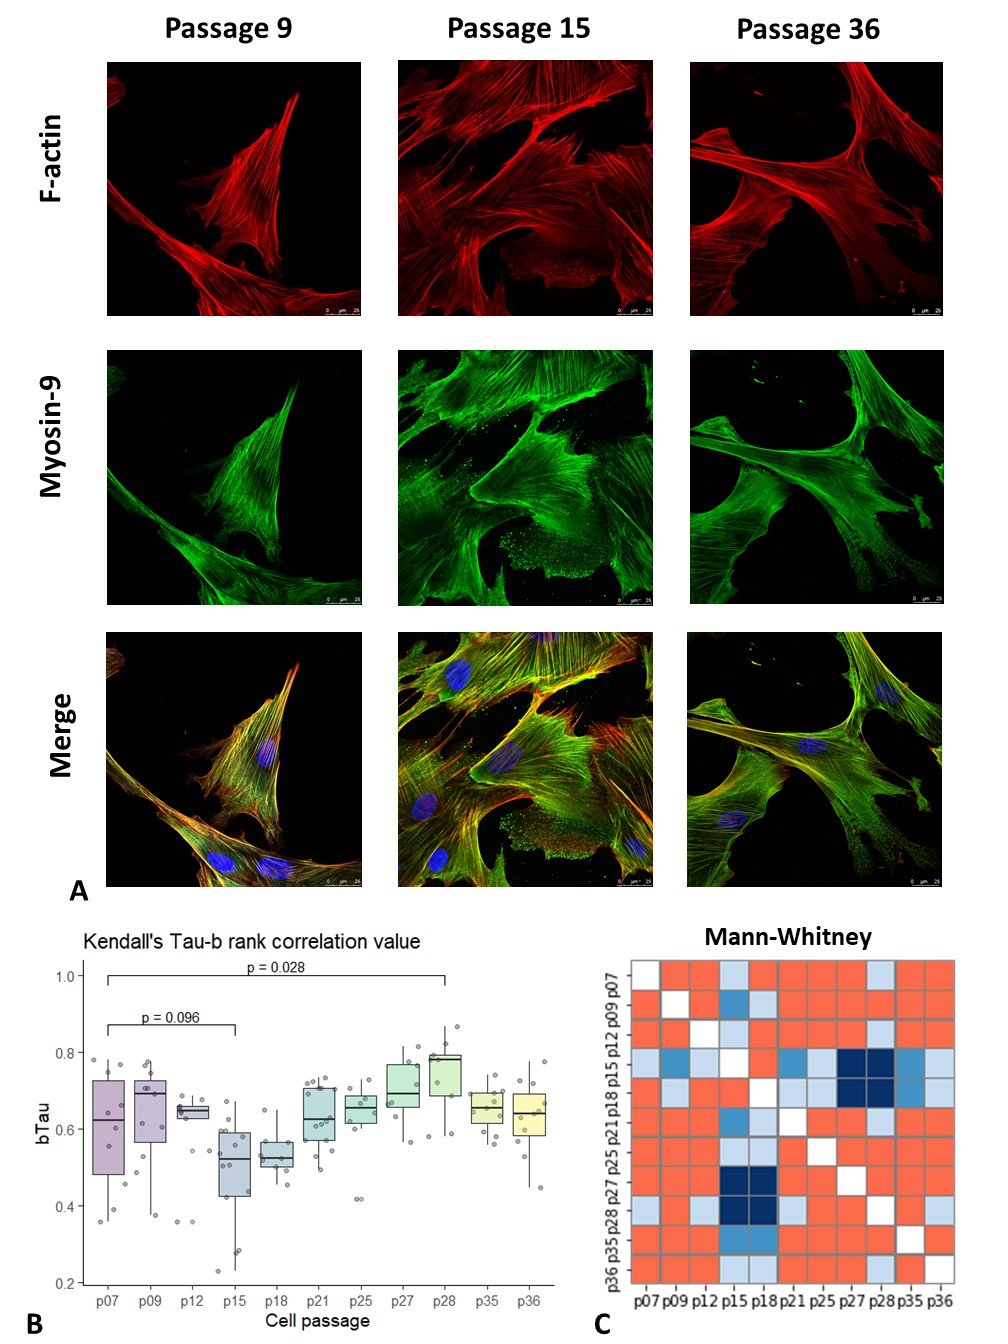
\includegraphics[width=0.9\linewidth]{myosin-9.jpg}
\caption{Fig. 1}
\end{figure}

\begin{figure}[hbt!]
\centering
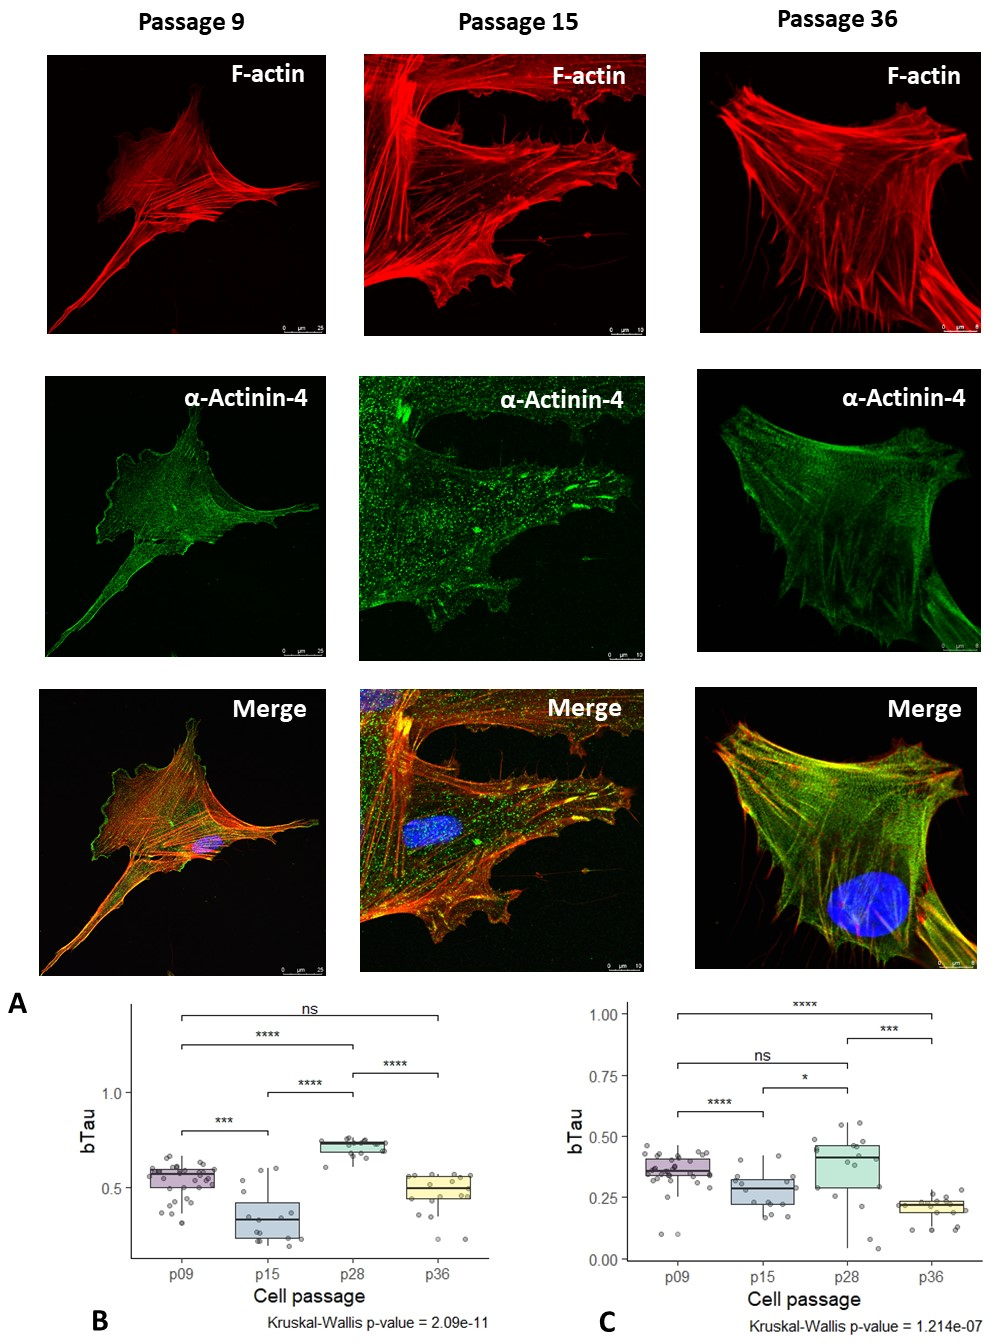
\includegraphics[width=0.9\linewidth]{alpha-actinin-4.jpg}
\caption{Fig. 2}
\end{figure}

\begin{figure}[hbt!]
  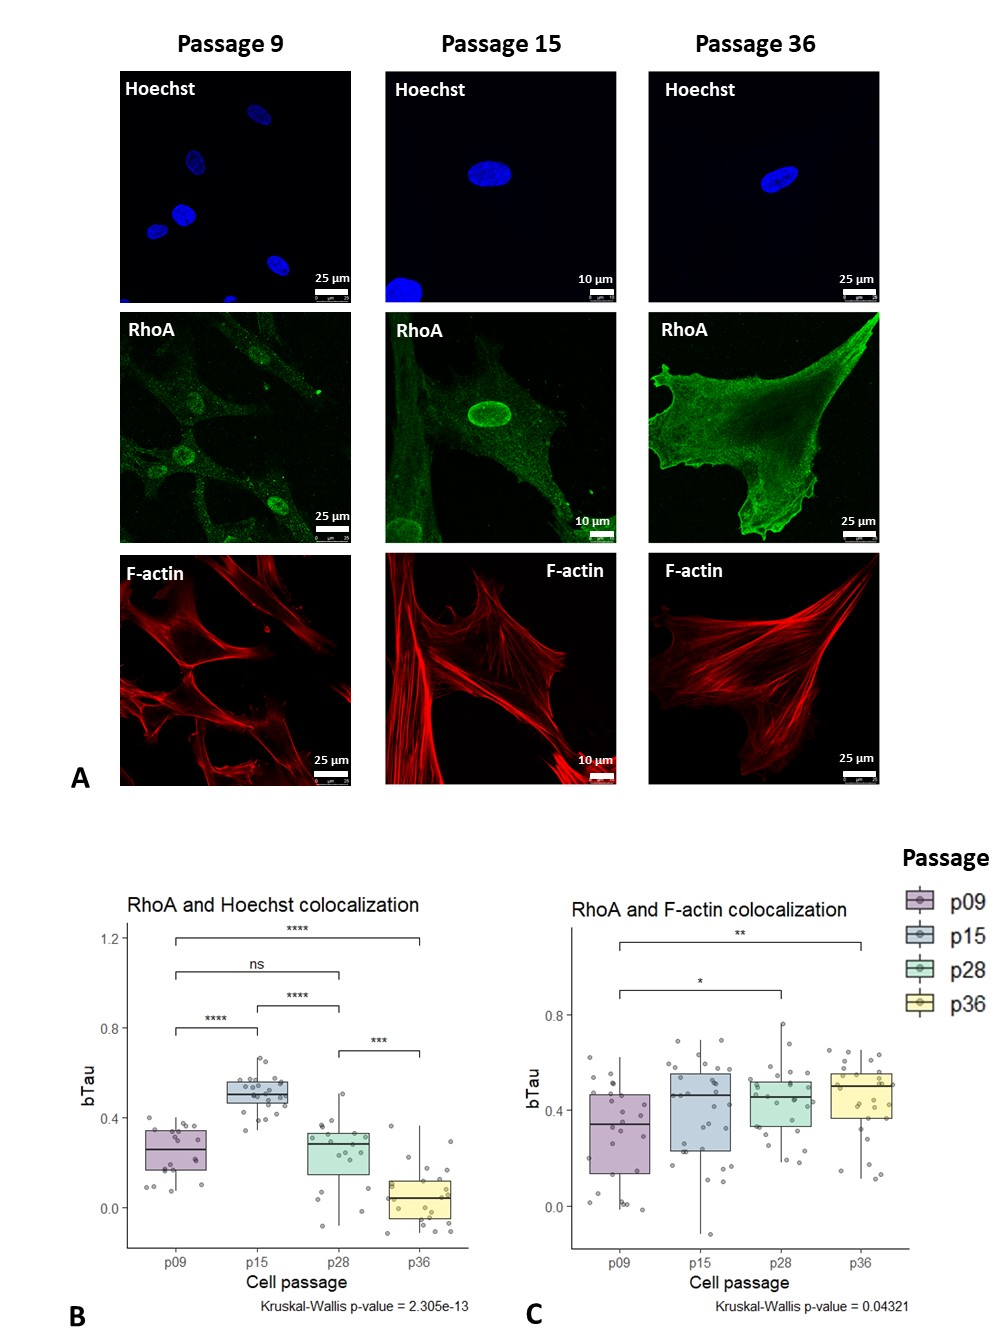
\includegraphics[width=0.9\linewidth]{rho.jpg}
  \caption{Fig. 3}
  \centering
\end{figure}

\begin{figure}[hbt!]
  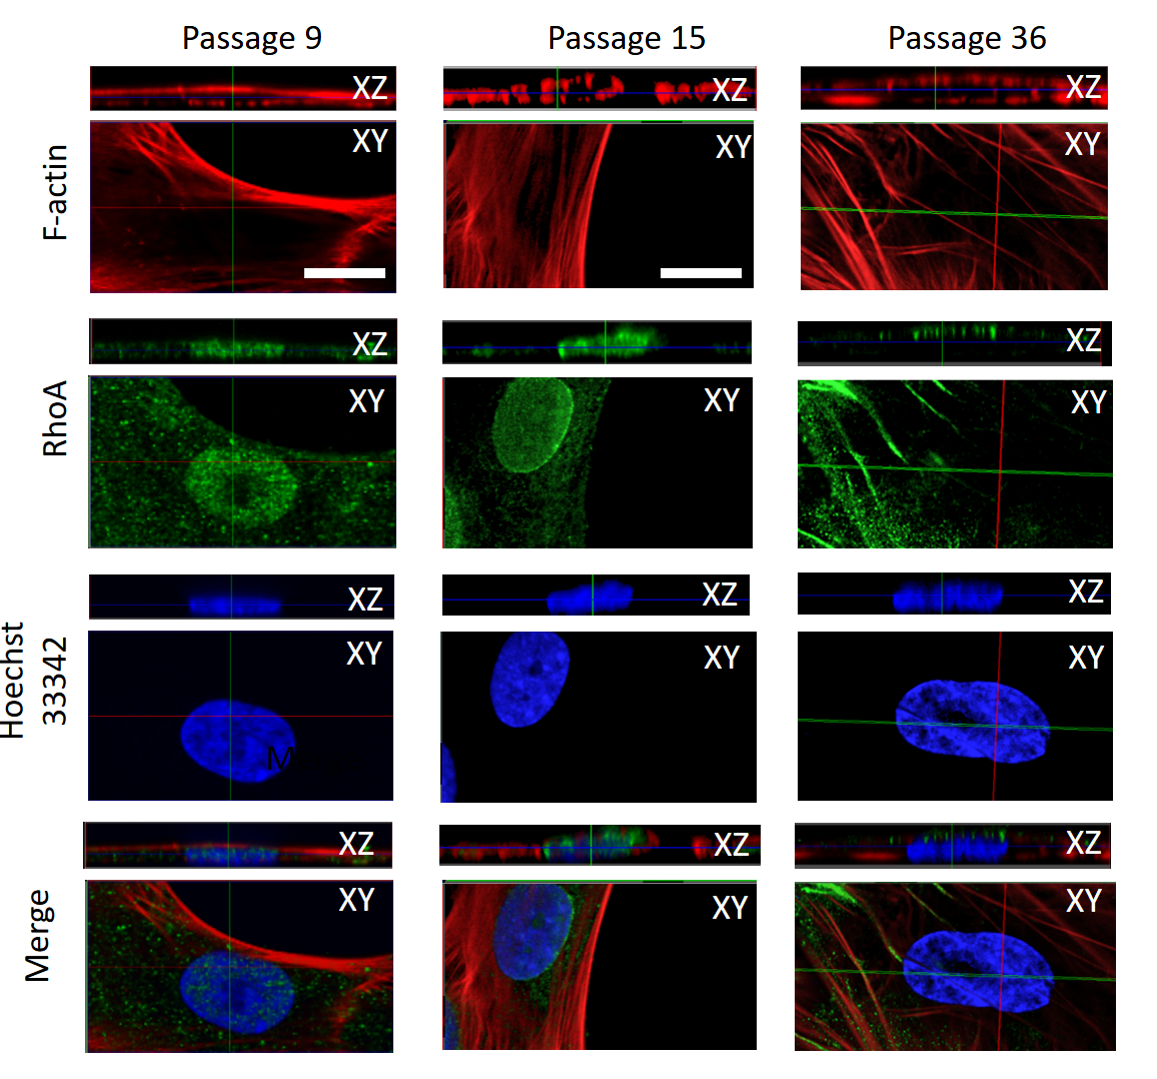
\includegraphics[width=0.9\linewidth]{rho-3d.png}
  \caption{Fig. 4}
  \centering
\end{figure}

\begin{figure}[hbt!]
  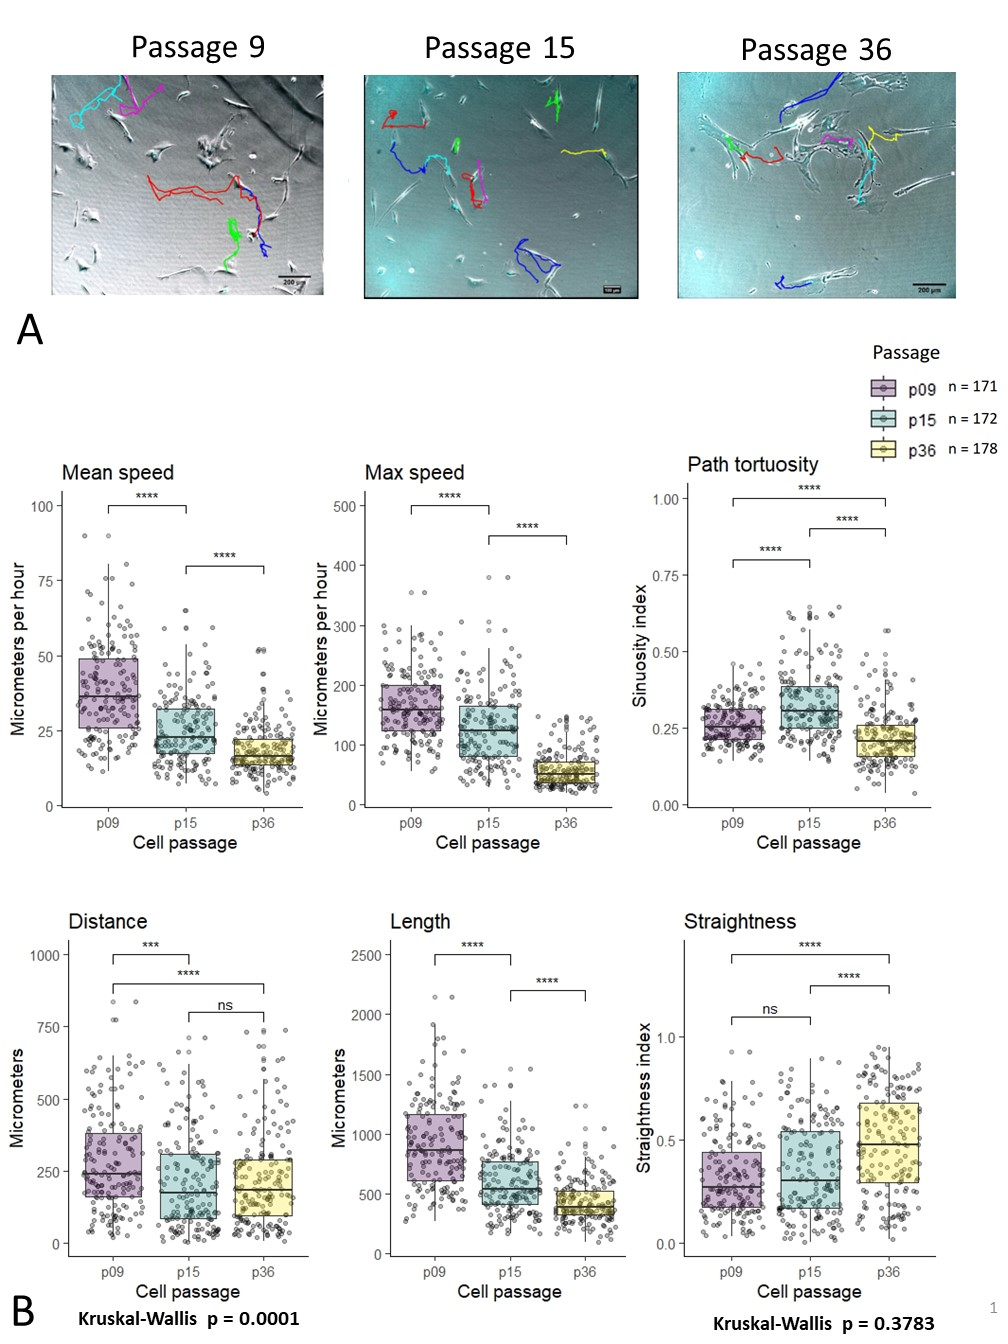
\includegraphics[width=1\linewidth]{traj.jpg}
  \caption{Fib. 5}
  \centering
\end{figure}

\begin{figure}[hbt!]
\centering
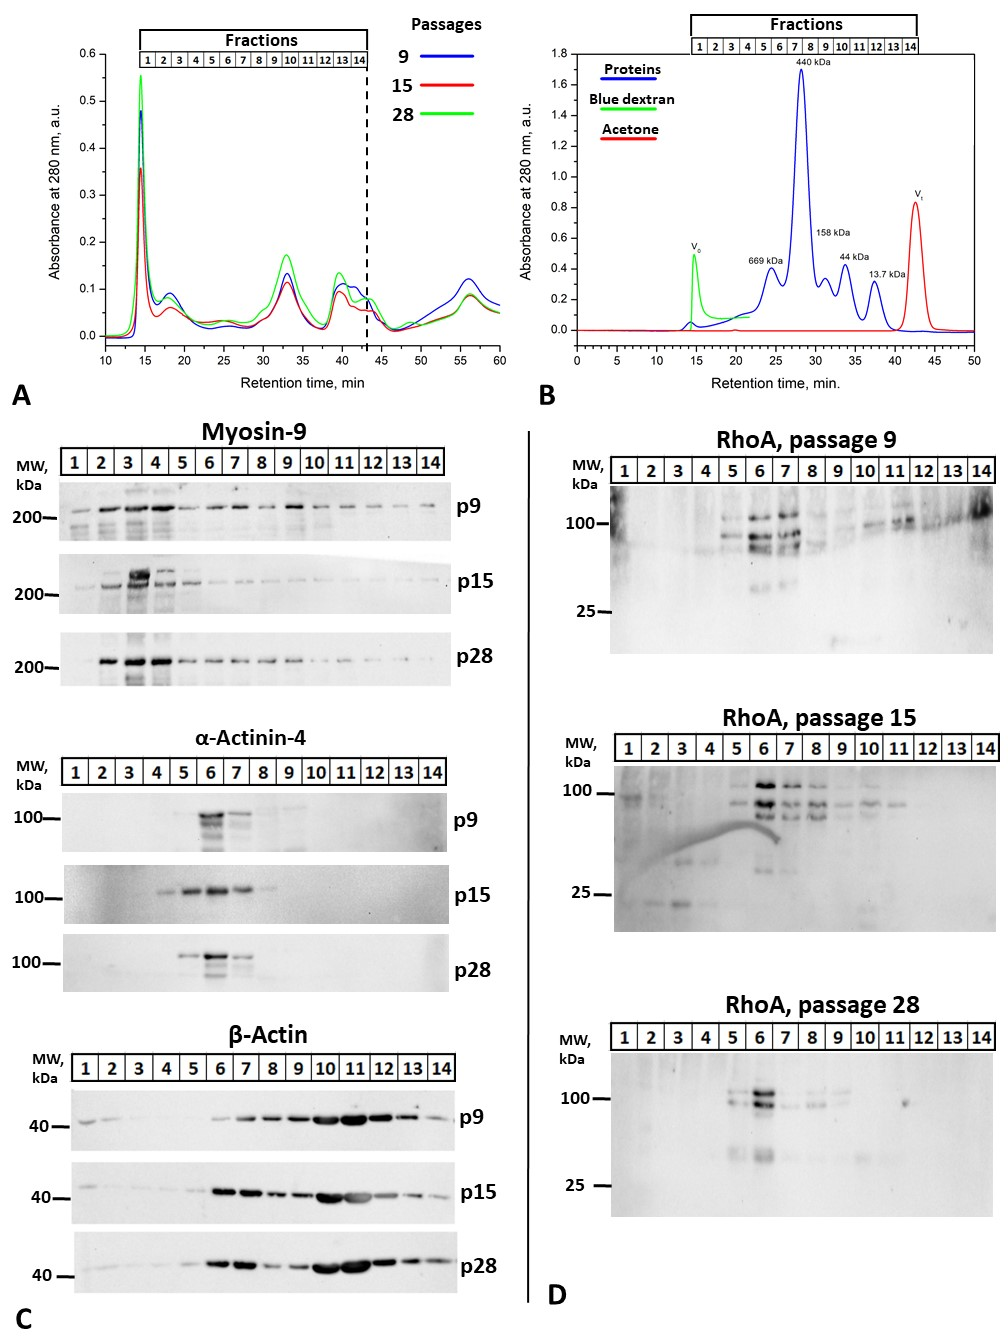
\includegraphics[width=1\linewidth]{fplc.jpg}
\caption{Fig. 6}
\end{figure}

\graphicalabstract{abstract}{We provide evidence for changes in the organization of the contractile apparatus of human mesenchymal stem cells in the process of replicative senescence.
The colocalization dynamics of of myosin-9 and alpha-actinin-4 with F-actin, as well as RhoA with nuclei, were studied at various passages during long cultivation of mesenchymal stem cells.
It was found that during replicative aging in MSCWJ-1 cells, a decline in cell speed and path tortuosity occurs.}

%\graphicalabstract{example-image-1x1}{Please check the journal's author guildines for whether a graphical abstract, key points, new findings, or other items are required for display in the Table of Contents.}

\end{document}
